% !TEX TS-program = pdflatex
% !TEX encoding = UTF-8 Unicode

% This is a simple template for a LaTeX document using the "article" class.
% See "book", "report", "letter" for other types of document.

\documentclass[11pt]{article} % use larger type; default would be 10pt

\usepackage[utf8]{inputenc} % set input encoding (not needed with XeLaTeX)

%%% Examples of Article customizations
% These packages are optional, depending whether you want the features they provide.
% See the LaTeX Companion or other references for full information.

%%% PAGE DIMENSIONS
\usepackage{geometry} % to change the page dimensions
\geometry{a4paper} % or letterpaper (US) or a5paper or....
% \geometry{margin=2in} % for example, change the margins to 2 inches all round
% \geometry{landscape} % set up the page for landscape
%   read geometry.pdf for detailed page layout information

\usepackage{graphicx} % support the \includegraphics command and options

% \usepackage[parfill]{parskip} % Activate to begin paragraphs with an empty line rather than an indent

%%% PACKAGES
\usepackage{booktabs} % for much better looking tables
\usepackage{array} % for better arrays (eg matrices) in maths
\usepackage{paralist} % very flexible & customisable lists (eg. enumerate/itemize, etc.)
\usepackage{verbatim} % adds environment for commenting out blocks of text & for better verbatim
\usepackage{subfig} % make it possible to include more than one captioned figure/table in a single float
\usepackage{graphicx} % can include graphics
\usepackage{float}
\usepackage{listings}
\usepackage{url}
\usepackage[spanish]{babel}
% These packages are all incorporated in the memoir class to one degree or another...

%%% HEADERS & FOOTERS
\usepackage{fancyhdr} % This should be set AFTER setting up the page geometry
\pagestyle{fancy} % options: empty , plain , fancy
\renewcommand{\headrulewidth}{0pt} % customise the layout...
\lhead{}\chead{}\rhead{}
\lfoot{}\cfoot{\thepage}\rfoot{}

%%% SECTION TITLE APPEARANCE
\usepackage{sectsty}
\allsectionsfont{\sffamily\mdseries\upshape} % (See the fntguide.pdf for font help)
% (This matches ConTeXt defaults)

%%% ToC (table of contents) APPEARANCE
\usepackage[nottoc,notlof,notlot]{tocbibind} % Put the bibliography in the ToC
\usepackage[titles,subfigure]{tocloft} % Alter the style of the Table of Contents
\renewcommand{\cftsecfont}{\rmfamily\mdseries\upshape}
\renewcommand{\cftsecpagefont}{\rmfamily\mdseries\upshape} % No bold!

%%% END Article customizations

%%% The "real" document content comes below...

\title{Lenguaje de programacion PHP}
\author{Lozano E. ,Lasso H. \& Alvarado L.}
%\date{} % Activate to display a given date or no date (if empty),
         % otherwise the current date is printed 

\begin{document}
\maketitle

\section{Introducción}
PHP es un lenguaje de programación definido para el desarrollo web de contenido dinámico y que se caracteriza por ser de código abierto. Sus siglas son un acrónimo recursivo de: “PHP: Hypertext Preprocessor” y actualmente ya en su quinta versión (PHP 5).
\\¿Qué hace a PHP importante? este lenguaje se ejecuta justo antes de enviar una página desde el servidor web a la ventana del usuario como vemos en la Figura \ref{fig:funcionamiento}, y su respuesta es una página en código HTML, he allí su compatibilidad con todos los navegadores, sistemas operativos y plataformas.  Es fácil de utilizar y con grandes ventajas como la gratuidad, independencia de plataforma, rapidez y seguridad. 

\begin{figure}[H]
  \centering
    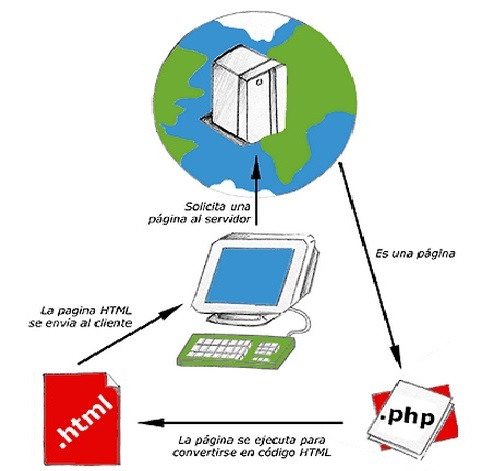
\includegraphics[width=0.4\textwidth]{Imagenes/diagrama-php}
  \caption{Esquema del funcionamiento de las páginas PHP}
  \label{fig:funcionamiento}
\end{figure}
 Y aunque este lenguaje tiene muchas ventajas, aun no se encuentra disponible un IDE con el cual mejorar su usabilidad; aunque igual trabaja muy bien y ha tomado así el papel principal del scripting (un lenguaje scripting es un tipo de lenguaje de programación que es generalmente interpretado) \cite{[1]}.

\section{Características}



\section{Historia}

Su creador fue  Rasmus  Lerdorf  quien nació en  Groenlandia  y cuya  profesión fue Ingeniero en Diseño de Sistemas Informáticos.En el año de 1994 Rasmus creó la primera versión de PHP, lo que quería era saber cuántas personas estaban leyendo su curriculum vitae en 
su página web , para poder realizar esto tuvo que crear  un   “Common Gateway Interface” en  Perl  que le revelaba  los resultados estadísticos en su propio sitio web.Rasmus el 8 de Junio de 1995 le puso como nombre a ese script PHP  “acrónimo de Personal Home Page”.

Dada a su gran aceptación Ramus decidió crear  un sistema para procesar formularios al que le puso el nombre de From Interpreter, y la unión de estas dos herramientas  se da  a cabo  la primera versión compacta del lenguaje :PHP/FI, cuya característica principal fue soporte interno para bases de datos, cookies y funciones definidas por el usuario.Una de las características de esta versión de PHP es proveer a los usuarios  una interfaz madura para múltiples bases de datos, protocolos, y APIs.

En 1997 debido a que PHP/FI era ineficiente y carente de las características que se requerían para impulsar una aplicación de comercio electrónico que estaban desarrollando para un proyecto de universidad.Andi Gutmans y Zeev Suraski discutieron varios aspectos de la implementación actual de PHP, decidieron mejorar el motor y comenzar a construir sobre las bases de PHP/FI existente, dando lugar a la creación de un nuevo e independiente lenguaje de programación este nuevo lenguaje fue publicado con el nombre de Hypertext  Preprocessor que es una nueva versión de PHP (PHP 3.0), en junio de 1998  PHP 3.0 fue anunciado por el nuevo equipo de Desarrollo de PHP como el descendiente oficial de PHP/FI 2.0.

En el invierno de 1998 Andi Gutmans y Zeev Suraski empezaron a trabajar en una nueva version de PHP, donde desarrollaron un nuevo motor llamado Motor Zend que viene de los nombres de pila Zeev y Andi.Una de la características importantes de esta versión es el soporte para la mayoría de servidores web, buffers de salida, sesiones HTTP y formas más seguras de controlar las entradas de usuarios.

Esta versión llamada PHP 4.0 fue publicada en Mayo del 2000 aproximadamente  dos años después que salió la versión PHP 3.0.
En la siguiente versión de PHP se trato de mejorar los mecanismos de la programación orientada a objetos dando como resultado un lenguaje más potente y que cada vez se hizo más popular, esta versión fue publicada en el año 2004 y se la llamo como PHP 5.0 
 

\section{Tutorial de Instalación}

\section{Hola Mundo y otros Programas Introductorios}
PHP es manejable cuando entendemos programación en HTML, ya que maneja conceptos conocidos como la cabecera (header), el cuerpo (body), etiquetas de apertura y cierre, entre otros. Y así seria un "Hola mundo" en PHP:

\begin{lstlisting}[frame=single]  % Start your code-block

<html>
    <head>
        <title>Ejemplo</title>
    </head>
    <body>
        <?php
            echo "Hola mundoooooo :D";
        ?>
    </body>
</html>
\end{lstlisting}
\begin{center}
Esquema del funcionamiento de las páginas PHP \cite{[2]}
\end{center}
Y así lo veriamos:
\begin{figure}[H]
  \centering
    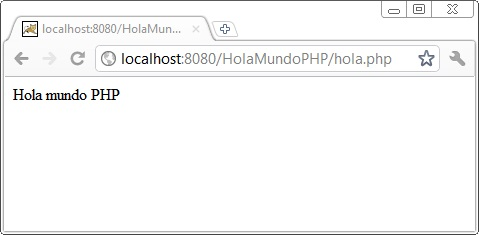
\includegraphics[width=0.5\textwidth]{Imagenes/HolaMundoPHP-Navegador}
  \caption{Un Hola Mundo con PHP}
  \label{fig:funcionamiento}
\end{figure}

\begin{thebibliography}{99}

\bibitem{[1]}  \textit Definición del Lenguaje Scripting [Online]. Available: \url{http://www.alegsa.com.ar/Dic/lenguaje%20scripting.php} Verificado: Octubre 21 - 2013
\bibitem{[2]}  \textsc{ PHP Group} \textit '¿Que es PHP?' [Online].Available: \url{http://php.net/manual/es/intro-whatis.php}  Verificado: Octubre 21 - 2013
\bibitem{[3]}  \textsc{ PHP Group} \textit Historia de PHP [Online]. Available \url{http://php.net/manual/es/history.php.php}  Verificado: Octubre 21 - 2013
\bibitem{[4]}  \textsc{ EcuRed} \textit PHP [Online]. Available \url{http://www.ecured.cu/index.php/PHP}  Verificado: Octubre 21 - 2013
\end{thebibliography}

\end{document}
